\chapter*{Ideas/Todos}

% \begin{marginfigure}
% 	\centering
% 	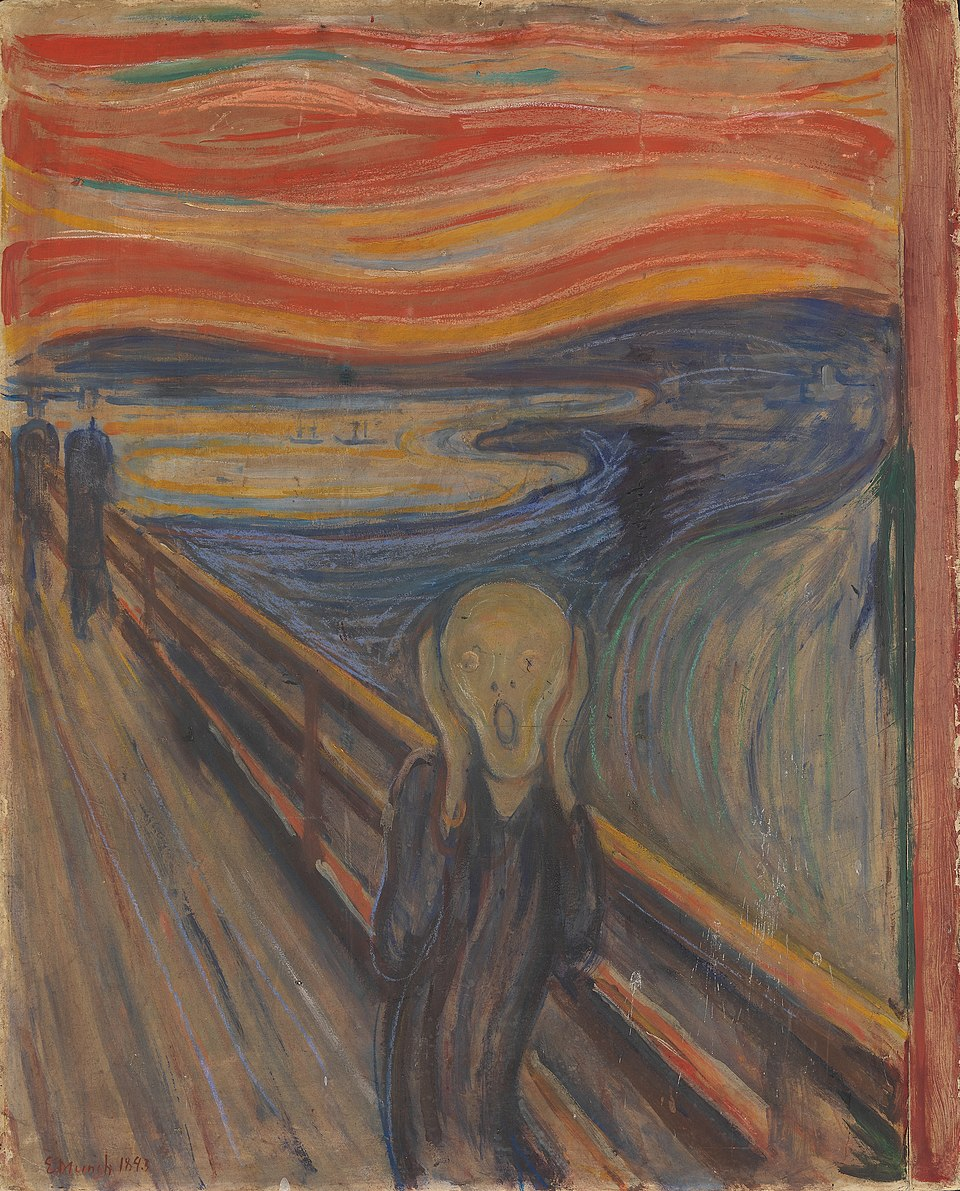
\includegraphics[width=\linewidth]{fig/prelim-db/Munch.jpg}
% 	\caption{
% 		When you learn that English has no word for ``epsilonesquement''
% 		two days before the final deadline for handing out your manuscript.
% 		\href{https://commons.wikimedia.org/wiki/File:Edvard_Munch,_1893,_The_Scream,_oil,_tempera_and_pastel_on_cardboard,_91_x_73_cm,_National_Gallery_of_Norway.jpg}{\emph{Skrik}},
% 		by Edvard Munch.
% 	}
% \end{marginfigure}

\begin{itemize}
	\item Clean intros/prelims \S~IV and \S~V.
	\item Duplicate label
	\item $\vertex{G} -> \vertex{\?G} -> G$…
	\item Use $\tup{}$ notation for tuples ("e.g." for "tagged tree decompositions")
	\item Cite ``TREE-WIDTH FOR FIRST ORDER FORMULAE''
	\item restatable in intro minimization
	\item Look at \cite{ChenGottlobLanzingerPichler2020Semantic}
	\item "homomorphic image" : check / move def
	\item add knowledge to abstracts
	\item query size macro ($|\Gamma|$ in stw)
	\item change proof sketch/proof to proof sketch/proof detail and check
		that there is no big overlap.
	\item Merge `app' of the two chapters
	\item look at sec-removed of minimization chapter
	\item unify atoms and vars command notations
	\item \todo{Change definition of CQ/CRPQ to have vertices. This allows for better duality,
		and also better statement for the Semantical Structure Theorem (in some prop we get
		``foo is an edge contraction of bla'' instead of ``is a minor of'').
		Update the definition of `one-way internal path' to allow for $n=0$.}
	\item \todo{allow autocite in margin.}
		\todo{citation at wrong place in margin.}
		\todo{do NOT overwrite options for sidenote, etc.}
		See \texttt{tufte-book-custom.cls}.
	\item \todo{Diego, biblio: ``some names have missing accents (esp polish), editors sometimes present sometimes not''}
	\item \todo{We/I!}
	\item \todo{Introduce $H^n_{\!\?A,\?B}$ notation for $\HCOperator^{\,n}_{\!\?A,\?B}(\topLatticeGuessFunctions{B})$.}
	\item \todo{Increase distance between footnote and figure caption}
	\item CQ x automatic (paper by Pablo I think)
\end{itemize}

At the end:
\begin{itemize}
	\item Check that figures are numbered by chapter (search for `Figure 1')
	\item fix breakline in toc of Chapter 1 for long section name
	\item check APs 
	\item O -> \backslash+O
	\item $\lBrack$ -> intInt amcro
	\item remove tags (\textsf{\backslash tag})
	\item mathbb -> symbb
	\item in bib: change inbook to incollection if no bookauthor entry
	\item check DOIs (no http), URL, consulted version, etc.
	\item \todo{replace all $\hdots$ (hdots) with $\dotsc$ (dotsc)}
	\item \todo{maximal under-approximation: des fois avec hyphen, des fois sans}
\end{itemize}

After submission:
\begin{itemize}
	\item \todo{improve negations: $A \nothomto B$ $\notFOmodels$ $\notcontained$
$\notFOmodels$ $\notcongr{\+R}$ $A \nothomregto B$}
\end{itemize}